\documentclass{beamer}

\usepackage[utf8]{inputenc}
\usepackage[brazil]{babel}
\usepackage{graphicx,hyperref,icmc,url}
\usepackage{subcaption}
\usepackage{multirow}
\usepackage{tikz}
\newcommand{\destaq}[1]{\textcolor{purple}{\textbf{#1}}}

% The title of the presentation:
%  - first a short version which is visible at the bottom of each slide;
%  - second the full title shown on the title slide;
\title[Reconstrução de curvas por características robustas extraídas de imagens]{Reconstrução de curvas por meio de características robustas extraídas de imagens}

% The author(s) of the presentation:
%  - again first a short version to be displayed at the bottom;
%  - next the full list of authors, which may include contact information;
\author[André Luís Mendes Fakhoury]{
    \Large{André Luís Mendes Fakhoury} \\ \medskip
    \small{\href{mailto:andrefakhoury@usp.br}{\nolinkurl{andrefakhoury@usp.br}}} \\ \bigskip
    \small{Orientador: João do Espirito Santo Batista Neto}
}

% \\ \bigskip
    % \large{}

% The institute:
%  - to start the name of the university as displayed on the top of each slide
%    this can be adjusted such that you can also create a Dutch version
%  - next the institute information as displayed on the title slide
\institute[ICMC/USP]{
    Vinculado ao Projeto Temático FAPESP: ``Mapeamento de características robustas entre diferentes domínios e espaços $\mathbb{R}^2$ e $\mathbb{R}^3$''\\ \medskip
    Instituto de Ciências Matemáticas e de Computação -- ICMC \\
    Universidade de São Paulo - USP
}

% Add a date and possibly the name of the event to the slides
%  - again first a short version to be shown at the bottom of each slide
%  - second the full date and event name for the title slide
\date[21/10/2021]{\footnotesize{21 de outubro de 2021}}

\AtBeginSection[]
{
    \begin{frame}<beamer>{Sumário}
        \tableofcontents[currentsection]
    \end{frame}
}

\begin{document}
    
    \begin{frame}[plain]
        \titlepage
    \end{frame}
    
    \begin{frame}
      \frametitle{Sumário}
      \tableofcontents
    \end{frame}
    
%%%%%%%%%%%%%%%%%%%%%%%%%%%%%%%%%%%%%%%%%%%%%%%%%%%%%%%%%%%%%%%%

\section{Contextualização} % intro do projeto e objetivos
\begin{frame}
\frametitle{Contextualização}

\begin{itemize}
\item \destaq{Mapeamento} de características robustas entre espaços bidimensionais e tridimensionais;
\item Simplificação através da \destaq{redução} da quantidade de informações.
\item \destaq{Características robustas:} características de uma superfície que se mantém quando esta se deforma \cite{book_difgeosing}. 
\end{itemize}

\end{frame}



\section{Métodos e procedimentos} % diagrama de atividades realizadas
\begin{frame}
\frametitle{Métodos e Procedimentos}
\framesubtitle{Visão geral}

\begin{figure}[hbt]
	\begin{center}
		\caption{Diagrama de bloco das etapas de desenvolvimento}
		\includegraphics[width=1\textwidth]{img/diagrama.png}
	\end{center}
\end{figure}

\end{frame}

% pre processamento
\subsection{Pré-processamento}

\begin{frame}
\frametitle{Pré-processamento}

\destaq{Objetivos:}
\begin{itemize}
\item Suavizar a imagem;
\item Remover ruídos.
\end{itemize}

\bigskip
\destaq{Técnicas utilizadas:}
\begin{itemize}
	\item Filtro gaussiano ou Perona-Malik;
	\item Binarização por Otsu;
	\item Operadores morfológicos (erosão e dilatação).
\end{itemize}
\end{frame}

\begin{frame}
\frametitle{Pré-processamento}

\destaq{Extração do contorno:}
\begin{itemize}
	\item Acompanha a borda do objeto, e verifica se seus vizinhos também pertencem ao objeto.
\end{itemize}

\begin{figure}[hbt]
	\begin{center}
		\caption{Método \textit{contour following}~\cite{book_shape}}
		\includegraphics[width=0.6\textwidth]{img/contorno.png}
	\end{center}
\end{figure}
\end{frame}

% calculo da curvatura + contorno
\subsection{Curvatura}

\begin{frame}
\frametitle{Escolha dos pontos}

\begin{itemize}
\item \destaq{Pontos linearmente espaçados:} índices igualmente espaçados entre si;
\medskip
\item \destaq{Escolha de pontos pela curvatura:} pontos com maior valor absoluto de curvatura.
\end{itemize}

\end{frame}

\begin{frame}
\frametitle{Curvatura}
\framesubtitle{Curvatura contínua}

Seja uma curva regular parametrizada por $t \rightarrow (x(t), y(t))$, em que $x(t)$ e $y(t)$ são funções de classe $C^2$. Sua curvatura é dada por:
$$\kappa (t) = \frac{x'(t) y''(t) - y'(t) x''(t)}{(x'(t)^2 + y'(t)^2)^{3/2}}$$   

\end{frame}


\begin{frame}
\frametitle{Curvatura discreta}
	
	No caso discreto, precisa-se calcular a derivada discreta.
	
	\medskip
	
	Utilização de \textbf{métodos espectrais de Fourier} \cite{brethwashington} e \textbf{filtro gaussiano} para suavizar e reduzir erros.
	
\end{frame}

\begin{frame}
\frametitle{Curvatura discreta}

Seja $u_j$ uma aproximação discreta da função $u(x)$, com $n$ pontos de amostra $x_j \in h, 2h, \dots, ih, \dots, 2\pi - h, 2\pi$, onde $h = 2\pi/n$. Pode-se aplicar a transformada rápida de Fourier (FFT) em $u_j$, tal que $FFT(u_j) \equiv \hat{u}_k$, em que $k \in \frac{-n}{2}+1, \dots, \frac{n}{2}$. Sabe-se que:

\medskip

$$FFT \left (\frac{\partial u_j}{\partial x} \right) \equiv i k \hat{u}_k$$

\medskip

Assim, para obter o valor da derivada, basta calcular a transformada rápida inversa IFFT.
\end{frame}


% reconstrucao - sorkine
\subsection{Reconstrução}

\begin{frame}
\frametitle{Reconstrução}
\framesubtitle{Definições}

\destaq{Modelagem geométrica:} conjunto de técnicas e algoritmos utilizados para modelar determinadas formas matemáticas, sujeitas a condições particulares de forma e suavidade.


\medskip
Uma forma possível de se modelar é com a utilização do \destaq{operador discreto de Laplace-Beltrami} \cite{Sorkine2006}.

\end{frame}

\begin{frame}
\frametitle{Coordenadas diferenciais}

Seja uma malha triangular $\mathcal{M} = (V, E, F)$. Cada vértice $\mathbf{v}_i \in V$ possui uma representação cartesiana dada por $\mathbf{v}_i = (x_i,y_i,z_i)$.

\medskip

\destaq{Coordenadas diferenciais} (ou $\mathbf{\delta}$\textit{-coordenadas}) de $\mathbf{v}_i$ são definidas como a diferença entre a coordenada cartesiana e o centro de massa de seus vizinhos imediatos na malha:

\begin{equation}
	\mathbf{\delta}_i = (\mathbf{\delta}_i^{(x)}, \mathbf{\delta}_i^{(y)}, \mathbf{\delta}_i^{(z)}) = \mathbf{v}_i - \frac{1}{d_i} \sum_{j \in N(i)} \mathbf{v}_j,
	\label{eq_delta}
\end{equation}

\noindent em que $N(i) = \{j|(i,j) \in E$\} e $d_i = |N(i)|$.

\end{frame}

\begin{frame}
\frametitle{Coordenadas diferenciais}
\framesubtitle{Transformação para $\delta$-coordenadas}

Seja $A$ a matriz de adjacências da malha:

$$
A_{ij} = \begin{cases}
	1&(i, j) \in E\\
	0&\text{caso contrário.}
\end{cases}
$$

e $D$ a matriz diagonal tal que

$$D_{ii} = d_{i} = |N(i)| = \text{número de vértices adjacentes a }i$$

A matriz $L$ de transformação de coordenadas cartesianas para as coordenadas diferenciais é:

\begin{equation}
	L = I - D^{-1}A.
\end{equation}

\end{frame}

\begin{frame}
\frametitle{Coordenadas diferenciais}
\framesubtitle{Transformação para $\delta$-coordenadas}

É mais comum utilizar a versão simétrica de $L$, $L_s$, tal que:

$$L_s = DL = D - A$$

e cada célula pode ser calculada por:

\begin{equation}
	(L_s)_{ij} = \begin{cases}
		d_i&i=j\\
		-1&(i, j) \in E\\
		0&\text{caso contrário.}
	\end{cases}
\end{equation}


\end{frame}

\begin{frame}
\frametitle{Coordenadas diferenciais}
\framesubtitle{Transformação para $\delta$-coordenadas}

Temos:

$$L_s \textbf{x} = \delta^{(x)}$$
$$L_s \textbf{y} = \delta^{(y)}$$
$$L_s \textbf{z} = \delta^{(z)}$$

e $L_s$ é denominado \destaq{Laplaciano topológico} da malha $\mathcal M$.

\end{frame}

\begin{frame}
\frametitle{Coordenadas diferenciais}
\framesubtitle{Discretização de Laplace-Beltrami}

Se considerar $\mathcal{M}$ uma aproximação linear por partes de uma superfície suave,

$$\delta_i = \frac{1}{d_i} \sum_{j \in N(i)}(\mathbf{v_i} - \mathbf{v_j})$$

é uma discretização de

$$\frac{1}{|\gamma|} \int_{v \in \gamma} (v_i - v) dl(v)$$

em que $\gamma$ é uma curva de uma superfície fechada simples em volta de $v_i$ e $|\gamma|$ é o comprimento de $\gamma$.

\end{frame}

\begin{frame}
\frametitle{Coordenadas diferenciais}
\framesubtitle{Discretização de Laplace-Beltrami}

Sabe-se que:

$$\lim\limits_{|\gamma|\rightarrow 0} \frac{1}{|\gamma|} \int_{v \in \gamma} (v_i - v) dl(v) = - H(v_i) n_i$$

em que $H(v_i)$ é a curvatura média de $v_i$ e $n_i$ é a normal à superfície.

\medskip

\begin{itemize}
	\item Intuitivamente, as $\delta$-coordenadas \destaq{encapsulam a forma local da superfície}:
	\begin{itemize}
		\item A direção aproxima o vetor normal;
		\item A norma aproxima a curvatura média;
	\end{itemize}
\end{itemize}

\end{frame}

\begin{frame}
\frametitle{Aplicações}
\framesubtitle{Representação eficiente de formas}

Com apenas informações de conectividade da malha e alguns pontos fixados (denominados vértices âncora), é possível aproximar toda a geometria, a partir da resolução do sistema pelo \destaq{método dos mínimos quadrados}:

\begin{equation}\label{eq:sisrecover}
	\left( \frac{L}{I_{m \times m} | 0} \right) \mathbf{x'} = \begin{pmatrix}
		0\\
		c_{1:m}^{(x)}
	\end{pmatrix}
\end{equation}

em que $c = \{v_1, v_2, \dots, v_m\}$ são os pontos âncora escolhidos como amostra.

\end{frame}

\section{Resultados}
\begin{frame}
\frametitle{Resultados}

\begin{itemize}
\item Imagens de folhas do repositório ImageCLEF (2011) \cite{imageclef2011};
\item Curvas em $\mathbb{R}^2$ e $\mathbb{R}^3$;
\item Malhas poligonais.
\end{itemize}
	
\end{frame}


\begin{frame}
\frametitle{Resultados}

\destaq{Cálculo do erro (distância euclidiana):}

\bigskip
Para cada vértice $i$, o erro dos pontos obtidos $\mathbf{v'}$ em relação aos pontos originais $\mathbf{v}$ é:

$$E_i(\mathbf{v, v'}) = \sqrt{(\mathbf v_i^{(x)} - \mathbf v_i'^{(x)})^2 + (\mathbf v_i^{(y)} - \mathbf v_i'^{(y)})^2}$$

\medskip

\noindent e o erro total da reconstrução é calculado como a soma do erro para cada ponto:

$$E(\mathbf{v, v'}) = \sum_{i = 1}^{|V|}E_i(\mathbf{v, v'})$$

\end{frame}


\begin{frame}
\frametitle{Resultados}
\framesubtitle{Imagens do banco de dados ImageCLEF (2011) \cite{imageclef2011}}
\begin{figure}[ht!]
	\centering
	\caption{Reconstrução em imagens de folhas.}
	\includegraphics[width=0.9\linewidth]{img/leaf_1.png}
	\includegraphics[width=0.9\linewidth]{img/leaf_2.png}
	\label{fig:leafs}
\end{figure}

\end{frame}


\begin{frame}
\frametitle{Resultados}
\framesubtitle{Curvas em $\mathbb{R}^2$ e $\mathbb{R}^3$}

\begin{figure}
	\centering
	\begin{subfigure}[b]{0.31\textwidth}
		\centering
		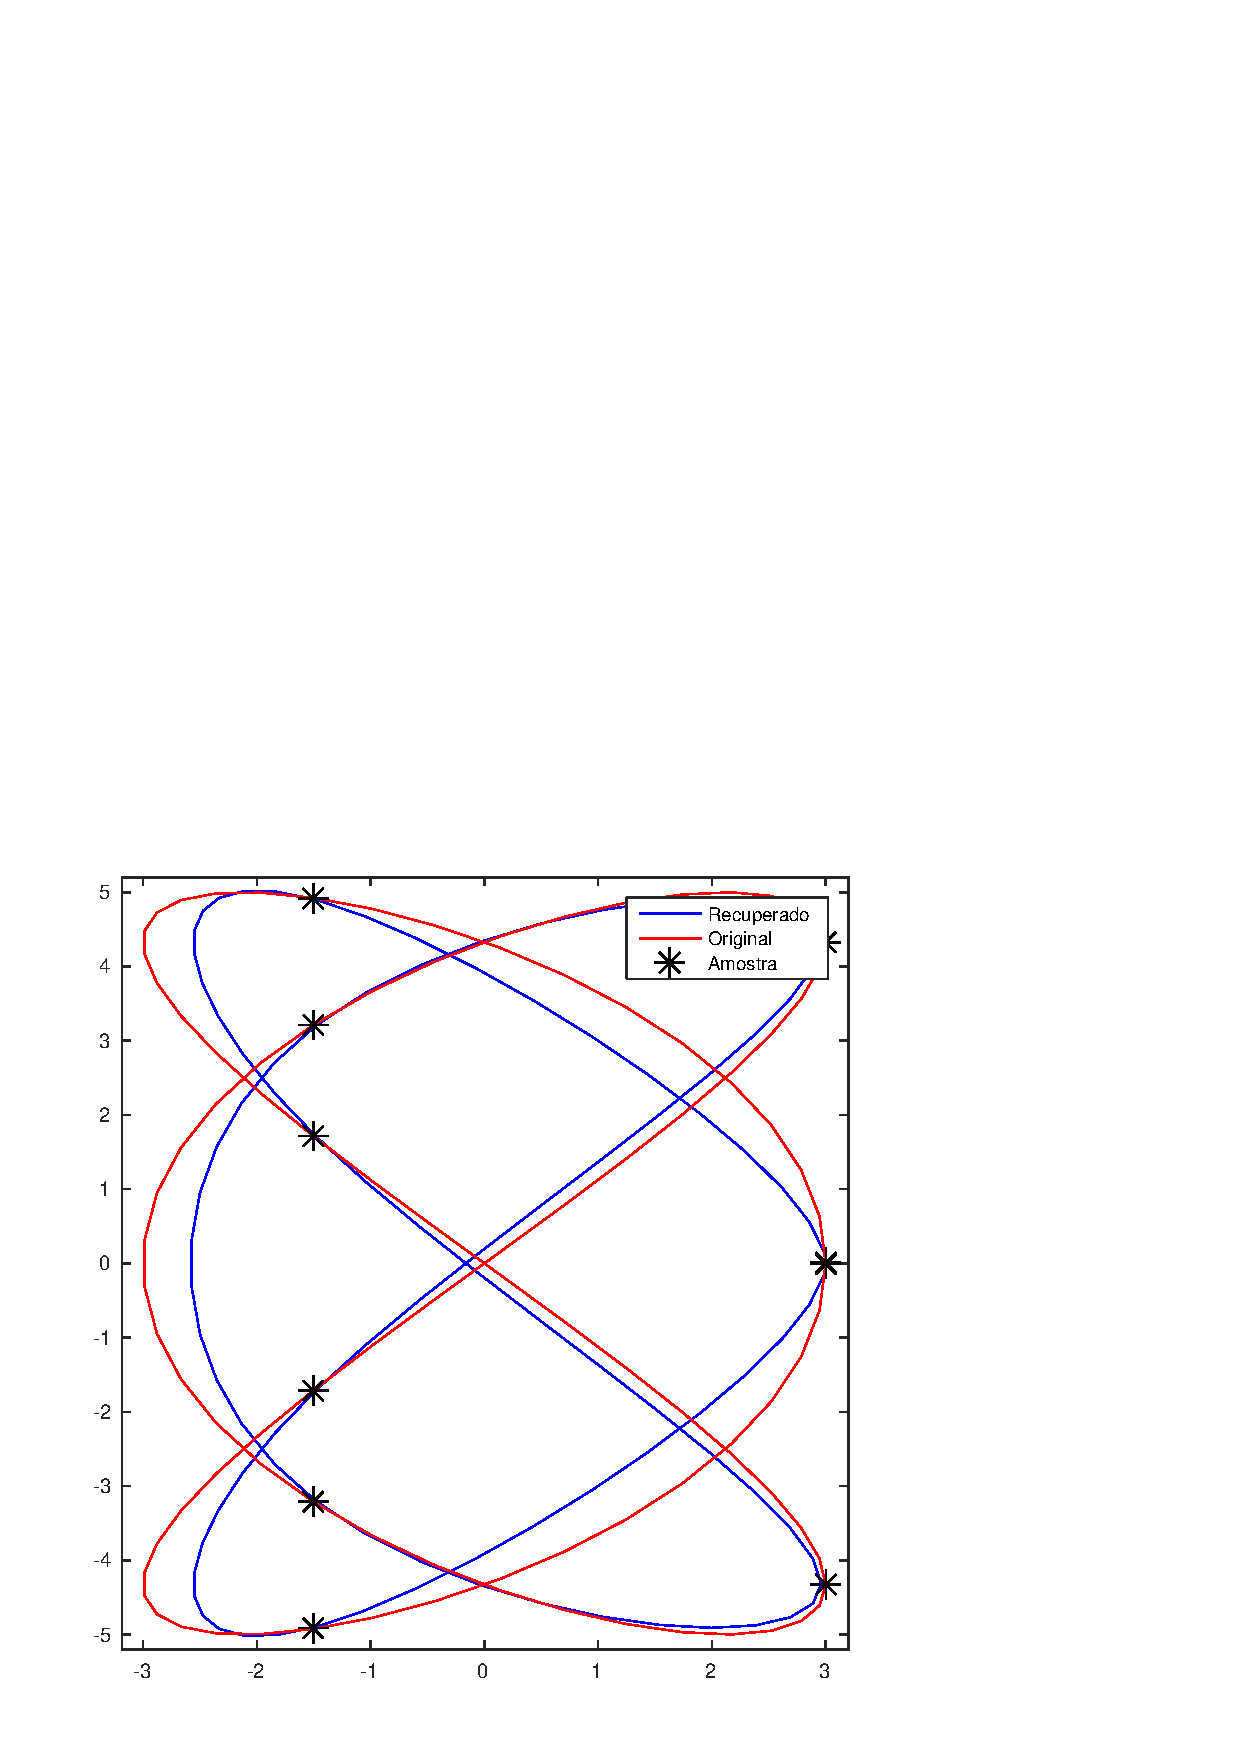
\includegraphics[trim={5cm 2cm 3cm 2cm},clip,width=\textwidth]{img/rep_2_10.jpg}
		\caption{10 pontos}
		\label{fig:ex24}
	\end{subfigure}
	\hfill
	\begin{subfigure}[b]{0.31\textwidth}
		\centering
		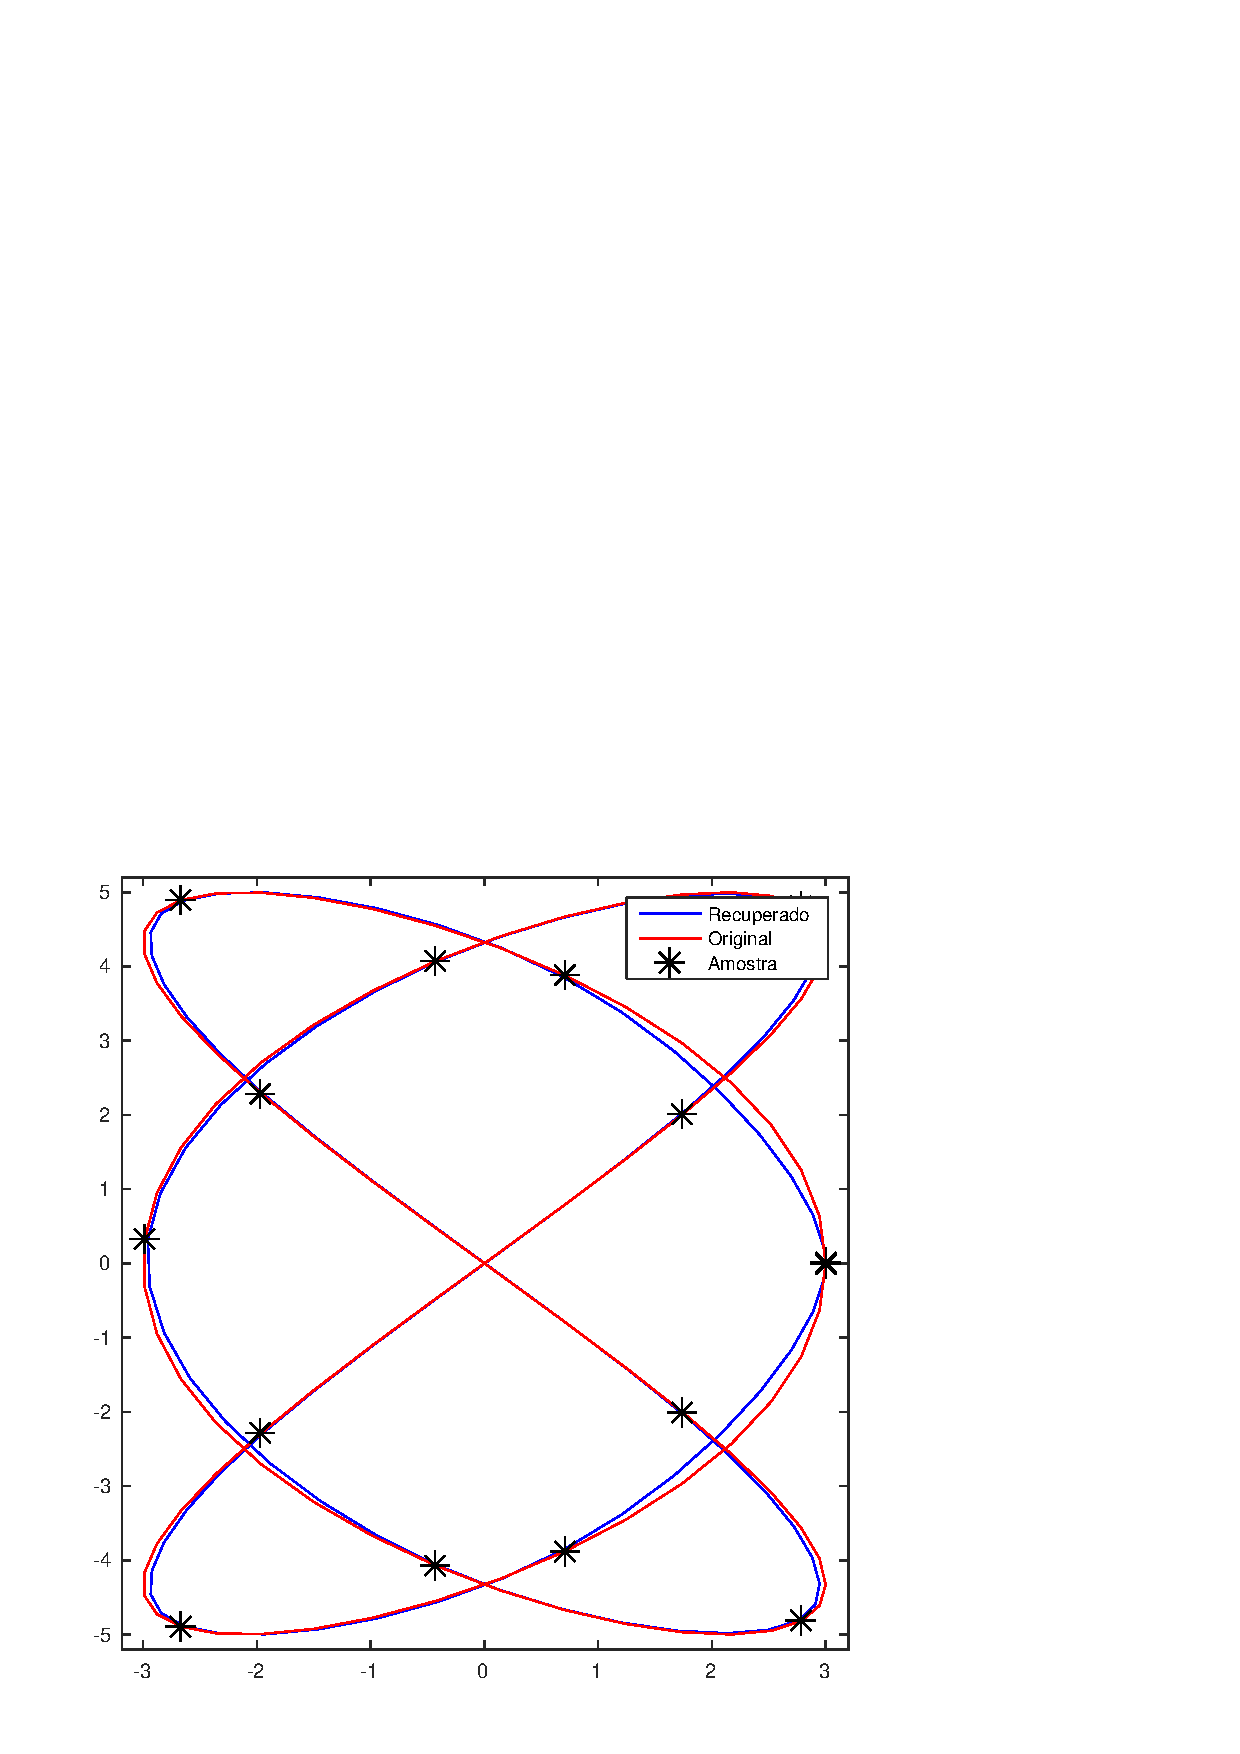
\includegraphics[trim={5cm 2cm 3cm 2cm},clip,width=\textwidth]{img/rep_2_15.jpg}
		\caption{15 pontos}
		\label{fig:ex22}
	\end{subfigure}
	\hfill
	\begin{subfigure}[b]{0.31\textwidth}
		\centering
		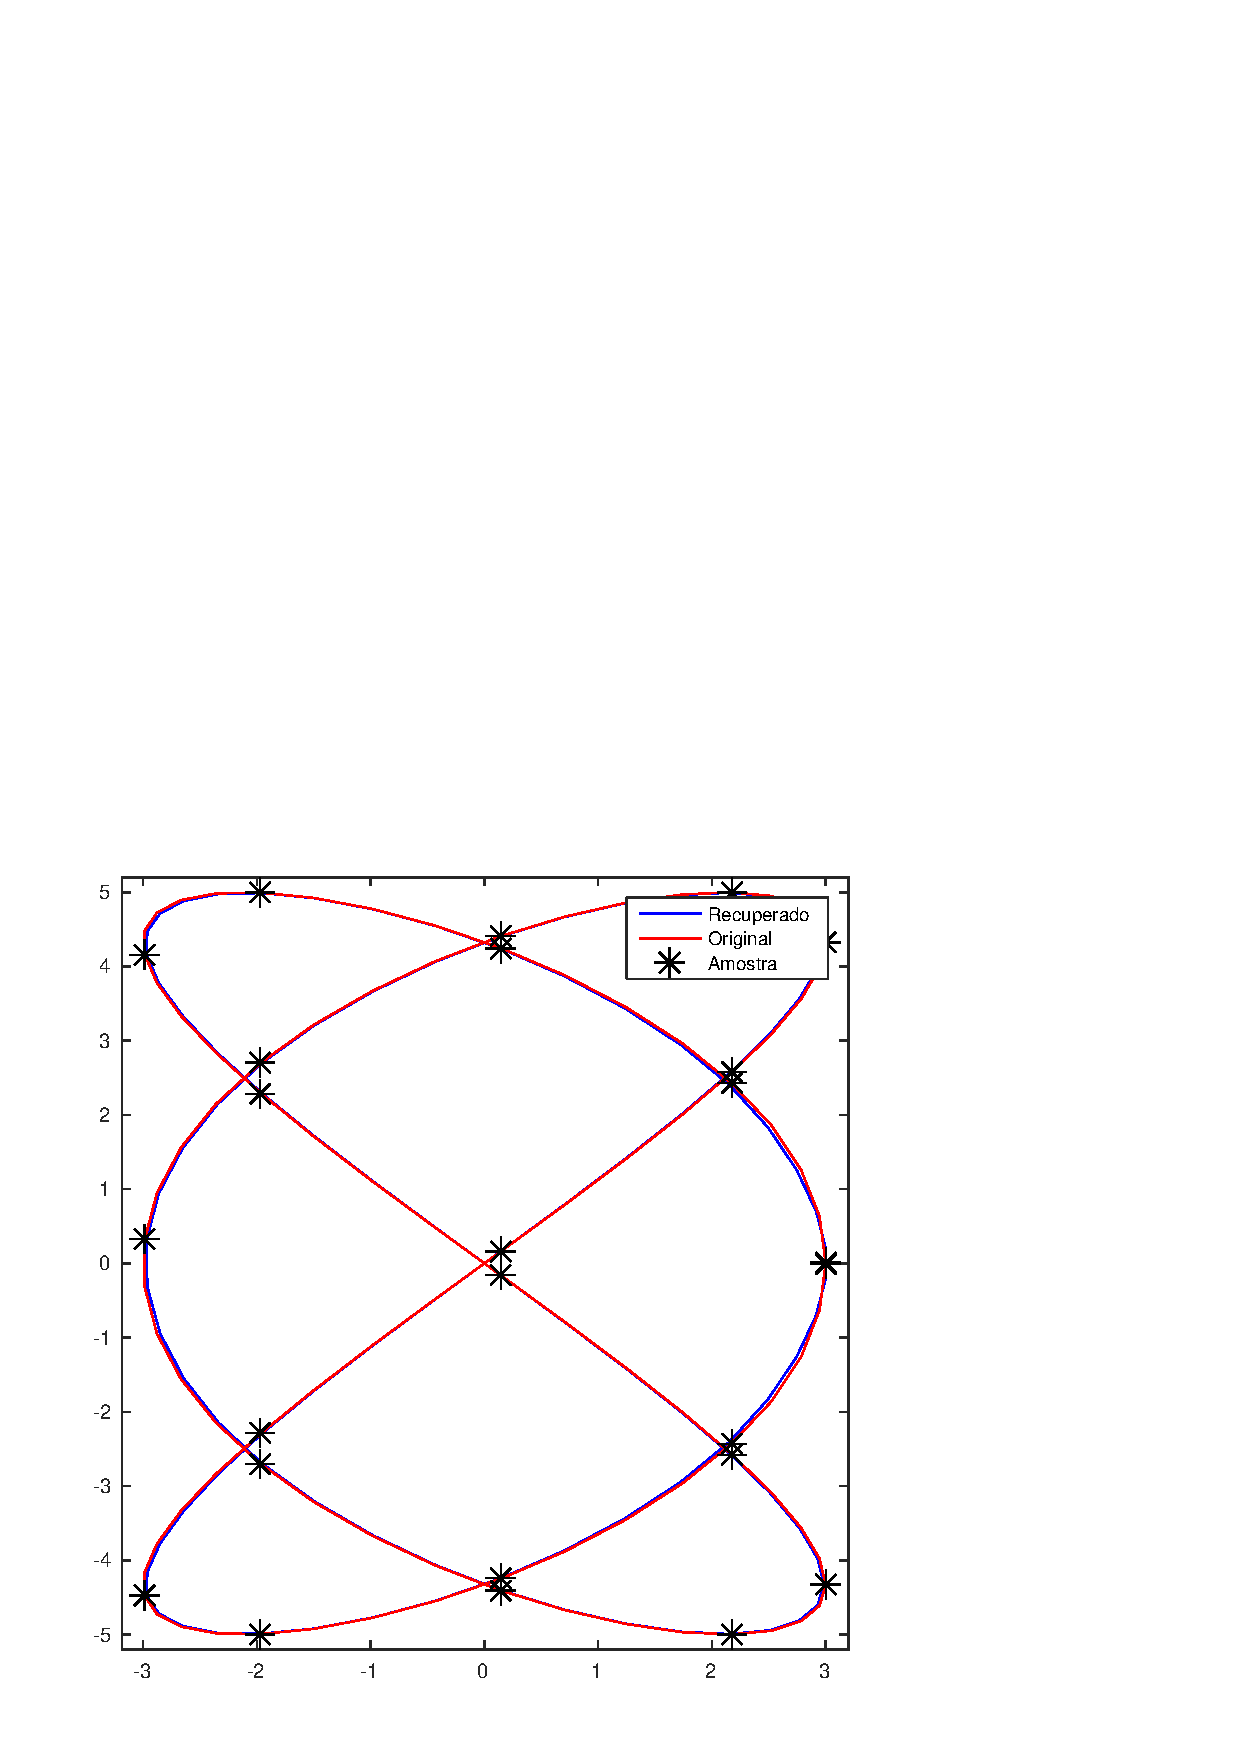
\includegraphics[trim={5cm 2cm 3cm 2cm},clip,width=\textwidth]{img/rep_2_25.jpg}
		\caption{25 pontos}
		\label{fig:ex23}
	\end{subfigure} %[3 * cos(3 * t); 5 * sin(2 * t)]';
	\caption{Representação da função paramétrica $(x(t), y(t)) = (3 cos(3t), 5sen(2t))$ utilizando alguns pontos igualmente espaçados como amostra.}
	\label{fig:ex2rep}
\end{figure}

\end{frame}


\begin{frame}
\frametitle{Resultados}
\framesubtitle{Malhas 3D}

\begin{figure}[hbt]
\begin{center}
	\caption{Representação da malha de um coelho}
	\includegraphics[width=0.45\textwidth]{img/mesh.png}
\end{center}
\end{figure}

\end{frame}




\section{Conclusão}
\begin{frame}
\frametitle{Conclusão}

A utilização do operador discreto de Laplace-Beltrami permite uma boa reconstrução, se forem utilizados pontos âncora suficientes e escolhidos de maneira correta (por exempo, pela curvatura). Porém alguns detalhes da malha original podem se perder, pois não serão considerados pelo algoritmo.

\end{frame}




%%%%%%%%%%%%%%%%%%%%%%%%%%%%
\section{Referências}

%\nocite{*}
\begin{frame}[allowframebreaks]
  \frametitle{Referência Bibliográfica}
  \bibliographystyle{siam}
  
  \bibliography{referencias}
\end{frame}

\end{document}
